\chapter{Introduction}
\label{chap:intro}

% motivation

Technology has automated an increasing variety of
difficult, dangerous, or menial tasks
previously performed by humans.
Computer algorithms now trade our stocks,
route our telephone calls and packages,
and fly our planes,
while simple machines clean our clothes and wash our dishes.
Recent advances may soon enable real-world nagivation applications
such as autonomous automobiles and drones.

More complex tasks require robots with many degrees of freedom.
Manipulation tasks, in particular,
present challenges in many areas including
perception, symbolic reasoning, and motion planning.
Successful applications have so far been largely
confined to large-scale manufacturing domains
whose prescribed and structured environments
allow these challenges to be overcome.

% narrow to motion planning more explicitly?
But what of applications such as
home assistance, disaster response, and small-batch manufacturing?
The robots of tomorrow will be required to plan
high-dimensional motions
in the face of geometrically complex and changing environments,
and do so under significant resource constraints.

% contributions

\vspace{0.2cm}
\begin{adjustwidth}{0.2in}{0.1in}
\emph{\large%
This thesis proposes an
efficient motion planning approach
well-suited
to articulated robots
performing recurring multi-step manipulation tasks
in complex, semi-structured environments.
}
\end{adjustwidth}
\vspace{0.2cm}

We begin by characterizing the challenges inherent in
motion planning for manipulation tasks.
We then detail a concerted set of insights which inform our approach.
The result is a collection of complementary algorithms
which together demonstrate that outperform
the current state-of-the-art.

\section{Problem Characterization}

Planning motions for articulated robots performing manipulation tasks
presents a number of challenges,
which we survey here.

A performant motion planner is only one component in a larger
robotic system,
which for many tasks must consider uncertainty, constraints,
motion control, and error recovery.

\paragraph{High Dimensionality.}
The continuous configuration spaces induced by robotic arms
often have higher dimensionality than typical vehicle navigation
problems.
Depending on the class of approach used,
this manifests itself as high branching factors
or costly nearest-neighbor queries,
and calls for intelligent discretization schemes.

\paragraph{Expensive Validity Checking.}
The robot and its environment are geometrically complex.
Homes and disaster areas are cluttered,
and arms with revolute joints render corresponding 
configuration space obstacles intractible to consider explicitly.
Further, since manipulation tasks require
motions that begin and end close to collisions with objects,
geometric models must have sufficiently high fidelity
to disambiguate feasible paths from colliding ones.
Testing candidate motions for collision therefore entails a
large computational cost during planning.

\paragraph{Planning vs. Execution Effort.}
The robot must allocate its limited resources
(e.g. time and energy) between planning motions and executing them.
To maximize task efficiency,
it is essential that motions be neither under-optimized
(leading to costly execution)
nor over-optimized (resulting in long planning pauses).
This balance is especially important for tasks with or around
humans,
who are particularly intolerant of both unpredictible motion
and planning pauses.

\paragraph{Semi-Structured Environments.}
The robot must continually generate planned motions in partially
changing environments.
This is especially evident when planning for manipulation tasks,
where each object grasp and placement changes the collision-free
subset of configuration space.

\begin{figure*}[t]
   \centering
   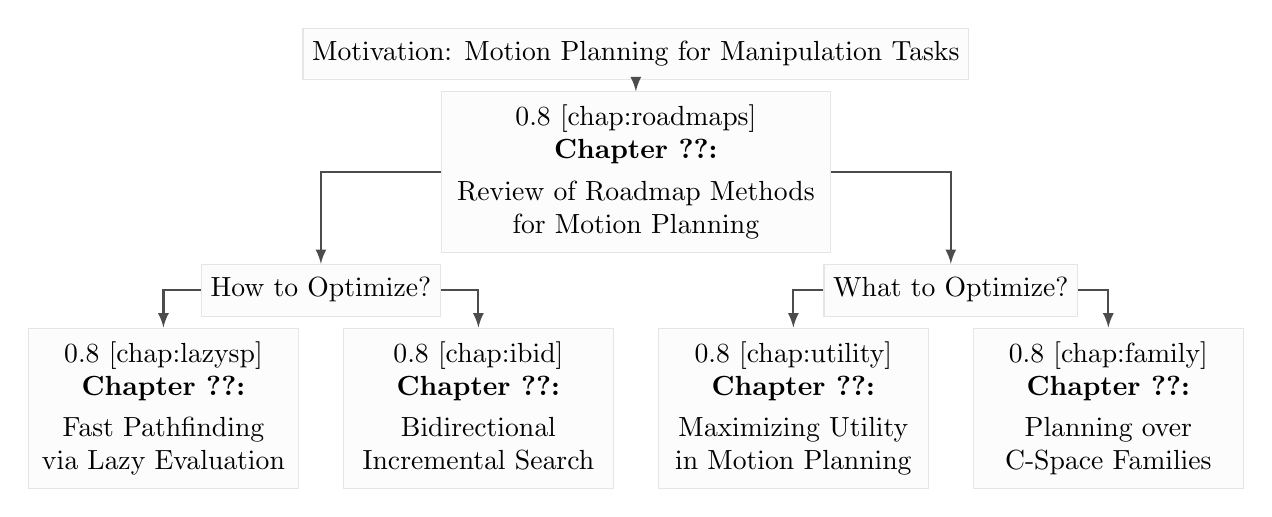
\begin{tikzpicture}
      \tikzset{>=latex} % arrow heads
   
      \node[draw=black!10,fill=black!1] (motiv) at ((0,0)
         {\strut Motivation: Motion Planning for Manipulation Tasks};

      \node[draw=black!10,fill=black!1] (roadmaps) at (0,-1.5) {\begin{minipage}{4.7cm}
         \vspace{0.05cm}\centering\setstretch{0.8}
         \hyperref[chap:roadmaps]{
         \strut {\bf Chapter~\ref{chap:roadmaps}:} \\
         \vspace{0.1cm} Review of Roadmap Methods for Motion Planning\strut
         }\end{minipage}};

      \node[draw=black!10,fill=black!1] (howopt) at (-4.0,-3.0) {\strut How to Optimize?};

      \node[draw=black!10,fill=black!1] (lazysp) at (-6.0,-4.5) {\begin{minipage}{3.2cm}
         \vspace{0.05cm}\centering\setstretch{0.8}
         \hyperref[chap:lazysp]{
         \strut {\bf Chapter~\ref{chap:lazysp}:} \\
         \vspace{0.1cm} Fast Pathfinding\\via Lazy Evaluation\strut
         }\end{minipage}};

      \node[draw=black!10,fill=black!1] (ibid) at (-2.0,-4.5) {\begin{minipage}{3.2cm}
         \vspace{0.05cm}\centering\setstretch{0.8}
         \hyperref[chap:ibid]{
         \strut {\bf Chapter~\ref{chap:ibid}:} \\
         \vspace{0.1cm} Bidirectional\\Incremental Search\strut
         }\end{minipage}};

      \node[draw=black!10,fill=black!1] (whatopt) at ( 4.0,-3.0) {\strut What to Optimize?};

      \node[draw=black!10,fill=black!1] (utility) at ( 2.0,-4.5) {\begin{minipage}{3.2cm}
         \vspace{0.05cm}\centering\setstretch{0.8}
         \hyperref[chap:utility]{
         \strut {\bf Chapter~\ref{chap:utility}:} \\
         \vspace{0.1cm} Maximizing Utility\\in Motion Planning\strut
         }\end{minipage}};

      \node[draw=black!10,fill=black!1] (family) at ( 6.0,-4.5) {\begin{minipage}{3.2cm}
         \vspace{0.05cm}\centering\setstretch{0.8}
         \hyperref[chap:family]{
         \strut {\bf Chapter~\ref{chap:family}:} \\
         \vspace{0.1cm} Planning over\\C-Space Families\strut
         }\end{minipage}};

      \draw[->,thick,black!70] (motiv) -- (roadmaps);
      \draw[->,thick,black!70] (roadmaps) -- (-4.0,-1.5) -- (howopt);
      \draw[->,thick,black!70] (roadmaps) -- ( 4.0,-1.5) -- (whatopt);
      \draw[->,thick,black!70] (howopt) -- (-6.0,-3.0) -- (lazysp);
      \draw[->,thick,black!70] (howopt) -- (-2.0,-3.0) -- (ibid);
      \draw[->,thick,black!70] (whatopt) -- ( 2.0,-3.0) -- (utility);
      \draw[->,thick,black!70] (whatopt) -- ( 6.0,-3.0) -- (family);

   \end{tikzpicture}
   \caption[][0.3cm]{Outline of the thesis document.
      Motivated by recurring manipulation tasks,
      we consider two questions:
      (a) how to optimize a motion planning objective
      over a C-space roadmap,
      and (b) which objective best captures
      the task's planning/execution tradeoff?}

   \label{fig:intro:outline}
\end{figure*}

\section{Outline of Approach}

This thesis develops an approach to motion planning
for articulated robots
which addresses these four challenges.
We provide an outline of the thesis in Figure~\ref{fig:intro:outline}.

\paragraph{\nameref{chap:roadmaps} (Chapter~\ref{chap:roadmaps})}
We begin by reviewing the definition of the motion planning problem
in terms of the robot's configuration space.
We examine several existing approaches from the literature,
including commonly-used sampling-based algorithms,
and discuss their various completeness and optimality properties.
We motivate our focus on the broad class of \emph{roadmap methods}
for solving the motion planning problem,
which allows it to be solved via pathfinding on a sequence of
progressively densified graphs
with a particular choice of edge weight function.
We also discuss the amenability of roadmap methods
to caching and parallelization.

\paragraph{\nameref{chap:lazysp} (Chapter~\ref{chap:lazysp})}
While roadmap methods effectively reduce the motion planning problem
to one of graph search,
the properties of the graph representation
(in particular, that evaluating an edge's weight entails costly
collision checks)
motivates a lazy approach to pathfinding.
Inspired by foundational algorithms
such as D* \citep{stentz1994dstar}
and the Lazy PRM \citep{bohlin2000lazyprm},
we introduce the \emph{Lazy Shortest Path (LazySP)} class of algorithms,
which relies on an inner incremental search algorithm
and can leverage an edge weight estimator. 
Importantly,
LazySP enables the a choice of \emph{edge selector},
which strongly influences pathfinding performance.
We introduce and compare various simple and novel selectors,
and show equivalences with existing algorithms
such as A* \citep{hart1968astar}
and Lazy Weighted A* \citep{cohen2014narms}.

\paragraph{\nameref{chap:ibid} (Chapter~\ref{chap:ibid})}
LazySP relies on an inner incremental search algorithm,
such as DynamicSWSF-FP \citep{ramalingam1996dynamicswsffp}
or Lifelong Planning A* \citep{koenig2004lpastar},
to nominate candidate paths on each iteration.
However,
the choices of selector and estimator strongly influence
the location of updated edges
and the vertex heuristic that can be used.
This motivates the development of a new search algorithm,
IBiD,
which combines bidirectional, heuristic, and incremental search
into a single generalized algorithm.

\paragraph{\nameref{chap:utility} (Chapter~\ref{chap:utility})}
Motion tasks expose a fundamental tradeoff between planning and
execution cost.
We show how conventional motion objective models
can be augmented to include a planning cost term,
and how such terms can be combined into a single measure of
\emph{utility},
which we can optimize explicitly
via particular weight/estimator functions using LazySP.
The resulting algorithm,
\emph{Lazily Evaluated Marginal Utility Roadmaps (LEMUR)},
demonstrates improved performance across a range of motion planning
queries
when compared to state-of-the-art planners.

\paragraph{\nameref{chap:family} (Chapter~\ref{chap:family})}
While utility maximization shows benefits in single-query settings,
many motion tasks (such as manipulation problems)
comprise multiple queries in a family of related configuration space
subsets.
We show how such problems can be formulated naturally via
augmented cost models with custom planning cost components.
We demonstrate improved performance in applications such as
cached checks and multi-step problems.

%Approach limitations: don't consider constraints,
%interleaved planning and execution, etc.
%Focus on kinematic problems.
%No uncertainty or feedback to symbolic planners.
%Complementary to many things.
%Deep dive.
%Part of a larger system.

\section{Summary of Contributions}

\begin{table*}[t]
   \centering
   {\renewcommand{\arraystretch}{1.4}
   \begin{tabular}{clll}
      \toprule
      Ch. & Problem & Algorithm & Description \\
      \midrule
      \ref{chap:lazysp} & Shortest Path (SP)
         & LazySP
         & {\renewcommand{\arraystretch}{0.8}%
            \begin{tabular}{@{}l@{}} Lazy search with edge selectors \\
            (induces an inner Dynamic SP problem)\end{tabular}} \\
      \ref{chap:ibid} & Dynamic Shortest Path
         & IBiD & Incremental Bidirectional Dijkstra's algorithm \\
      \ref{chap:utility} & Motion Planning
         & LEMUR
         & {\renewcommand{\arraystretch}{0.8}%
            \begin{tabular}{@{}l@{}} Lazily Evaluated Marginal Utility Roadmaps \\
            (accepts a domain-specific cost model)\end{tabular}} \\
      \ref{chap:family} & Family Motion Planning
         & Family LEMUR
         & Express a C-space family as a LEMUR cost model \\
         %LEMUR over a family of C-space subsets \\
      \bottomrule
   \end{tabular}}
   \caption[][0.5cm]{Table of algorithms developed in this thesis.}
   \label{table:intro:table-of-algorithms}
\end{table*}

We summarize the contributions of this thesis here.
A table of the developed algorithms is presented in
Table~\ref{table:intro:table-of-algorithms}

\begin{itemize}
\item The LazySP pathfinding algorithm for graphs with expensive
   edge evaluations,
   along with accompanying novel edge selectors.
\item The IBiD bidirectional, heuristic, incremental search algorithm.
\item The LEMUR algorithm for maximizing utility
   in motion planning problems.
\item Formulation of the C-space family motion planning problem,
   and application of LEMUR to it.
\item An experimental evaluation of the above algorithms against a
   selection of motion planning tasks.
\item Open-source implementations of the above algorithms for the
   Boost Graph Library (BGL) \citep{siek2001boostgraph},
   Open Motion Planning Library (OMPL), \citep{sucan2012ompl}
   and OpenRAVE \citep{diankov2010openrave} software packages.
\end{itemize}

\cdnote{Maybe talk more about different applications /
   expensive edge validation /
   the relationship between lazy and dynamic search / etc?}

%While well-suited for arms,
%the contributions are relevant more broadly.
%Other applications.
%Pathfinding algorithms.

\section{Review of Experimental Platforms and Problem Instances}

\begin{figure*}[t]
   \centering
   
   \subfloat[The HERB home robot experimenal platform.]{%
      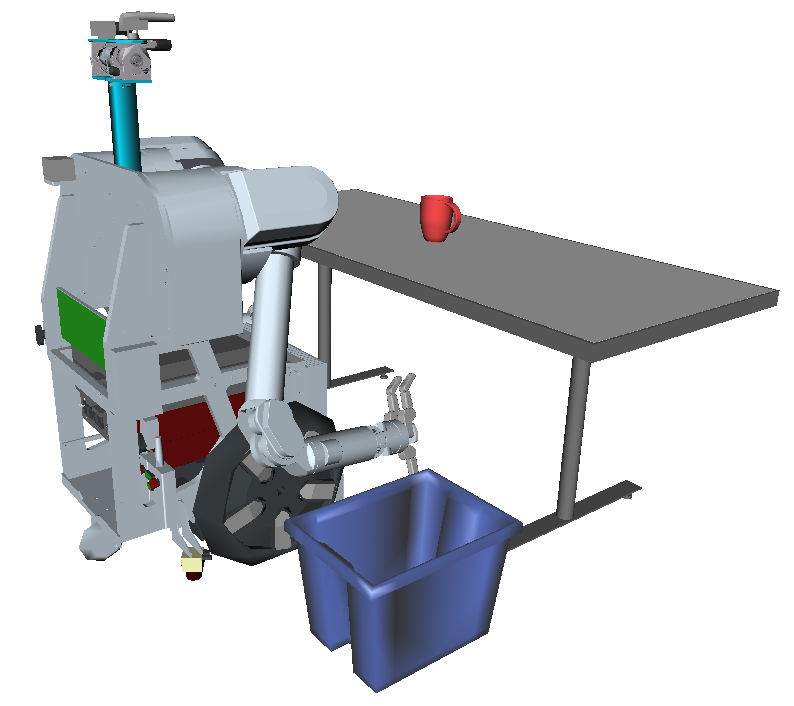
\includegraphics[height=3.25cm]{figs/simple-table-clearing-task.png}
      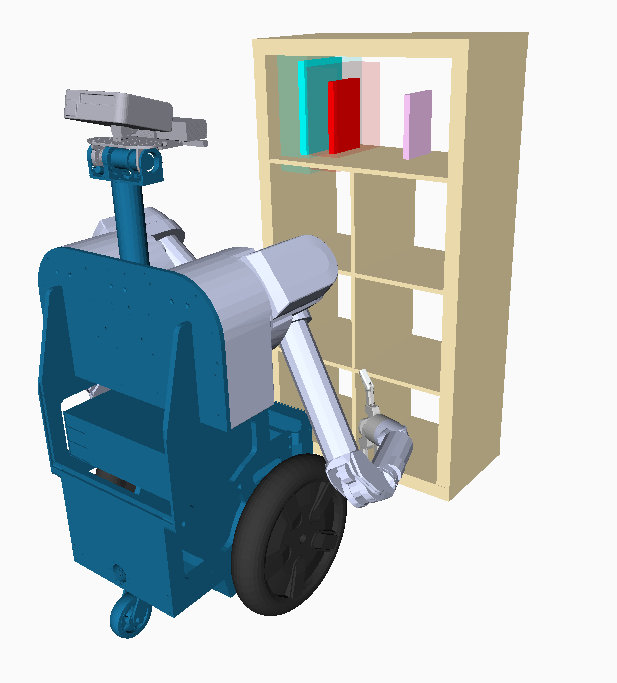
\includegraphics[height=3.25cm]{figs/herbarm-traj0-t000.png}
      \label{subfig:intro:platform-herb}
   }%
   \quad%
   \subfloat[An ABB IRB 440 robot in an industrial workcell.]{%
      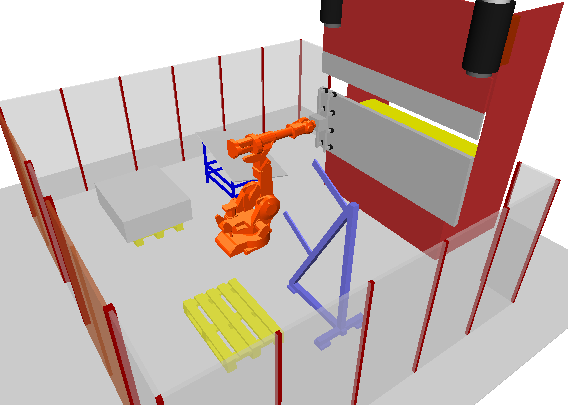
\includegraphics[height=3.25cm]{figs/workcell/config-a.png}
      \label{subfig:intro:platform-irb4400}
   }%
   \quad%
   \subfloat[The CHIMP disaster response robot.]{%
      \quad%
      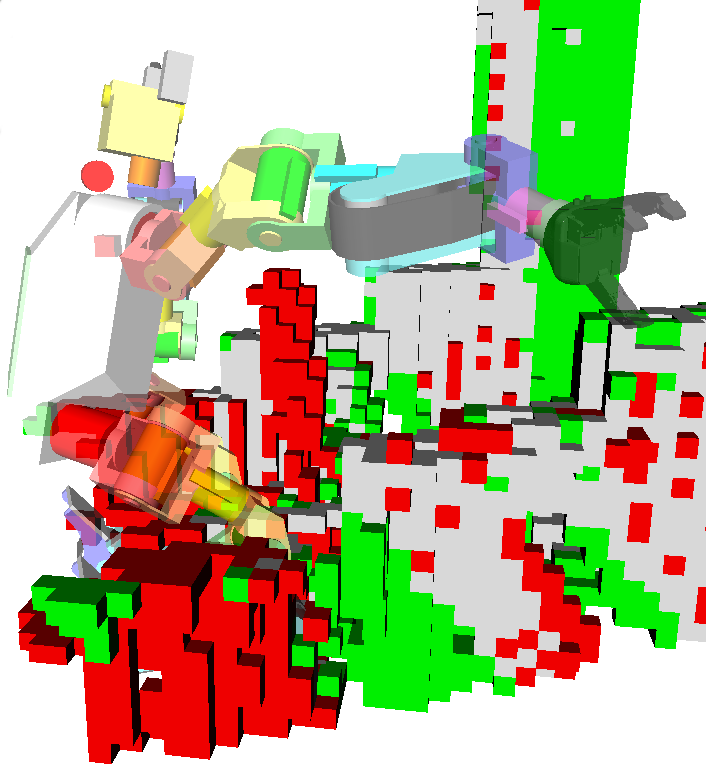
\includegraphics[height=3.25cm]{figs/chimp-voxels-delta.png}%
      \quad
      \label{subfig:intro:platform-chimp}
   }%
   
   \caption[][0.5cm]{Robotic platforms considered in this thesis.}
   \label{fig:intro:platforms}
\end{figure*}

We consider a number of motion and manipulation planning instances
across three robotic platforms:
\begin{itemize}
\item Figure~\ref{fig:intro:platforms}\subref{subfig:intro:platform-herb}:
   HERB, the Home Exploring Robot Butler
   \citep{srinivasa2012herb20}.
\item Figure~\ref{fig:intro:platforms}\subref{subfig:intro:platform-irb4400}:
   IRB 4400, a compact industrial robot from ABB.
\item Figure~\ref{fig:intro:platforms}\subref{subfig:intro:platform-chimp}:
   CHIMP, the CMU Highly Intelligent Mobile Platform
   \citep{stentz2014chimp}.
\end{itemize}

\cdnote{Forward ref to experimental evaluation sections.}
